\section{Methodology \& Planning}
\subsection{Methodology}
For any kind of development it's important to have a plan of how the software is going to take shape and progress as it goes on. 

This project will be designed in iterative stages with a feedback loop so the project is dynamic and can change direction as research and other area's are finalised. In addition it's important to choose a methodology that is not heavy on design and documentation, having this trait allows the system to be developed quickly. The best suited methodologies for both of these scenarios are Extreme Programming (XP) and Rapid Application Development (RAD). One important thing about both of these methodologies is the fact they have a feedback loop , this feedback loop will allow the project to stay pliable and adapt as needed, the feedback is normally supplied by a stakeholder but in the case of this project the author, project supervisor and second marker will act as a stakeholder. Finally as both of these methodologies are well known and compared online no direct comparison will be made of these, however Figure \ref{fig:xp} and \ref{fig:rad} contain the base principal of these methodologies.

\begin{figure}[h]
	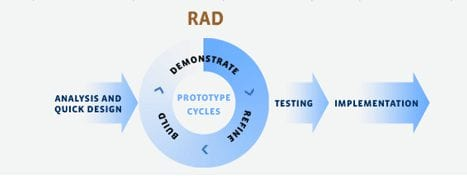
\includegraphics[width=\linewidth]{./images/methodology/RAD.png}\\
	\caption{Rapid Application Development (\cite{ankitasingh_2019_what})}
	\label{fig:rad}
\end{figure}
\begin{figure}[h]
	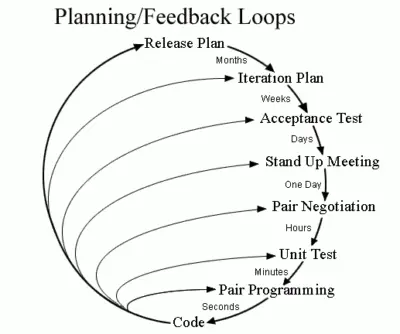
\includegraphics[width=0.5\linewidth]{./images/methodology/XP.png}\\
	\caption{Extreme Programming (\cite{ponomareff_learning})}
	\label{fig:xp}
\end{figure}


As mentioned above the chosen methodology needs to have a priority on quick development part of this is due to the limited time of the project overall. RAD is a methodology specifically designed for this use however it does have some well known caveats such as the bad quality of code it produces due to lack of testing and the emphasis on quick development, this is briefly covered by (\cite{kissflow_2019_rapid}). XP is designed to be a team based methodology so doesn't directly fit into a solo project, such as stand-ups, pair programming etc. However elements such the unit testing are an excellent stage of development. For this reason a combination of the 2 will be used where as part of the RAD cycle Unit Tests \& acceptance testing are added. This makes the overall time spent longer however improves the quality of the project and allows it to still be pliable in the direction as it progresses.
\pagebreak
\subsection{Planning}
A project plan has been developed listing the key milestones intended for the project over the year see figure \ref{fig:projlan}. Details are lacking on this plan, and instead list target goals. Goals will be generated daily/weekly to direct towards each target via a Kahnbahn board or to-do list, using this approach allows for good use of the agile methodology and easy changing of priorities or order in accordance to the general plan.

\begin{figure}[h]
	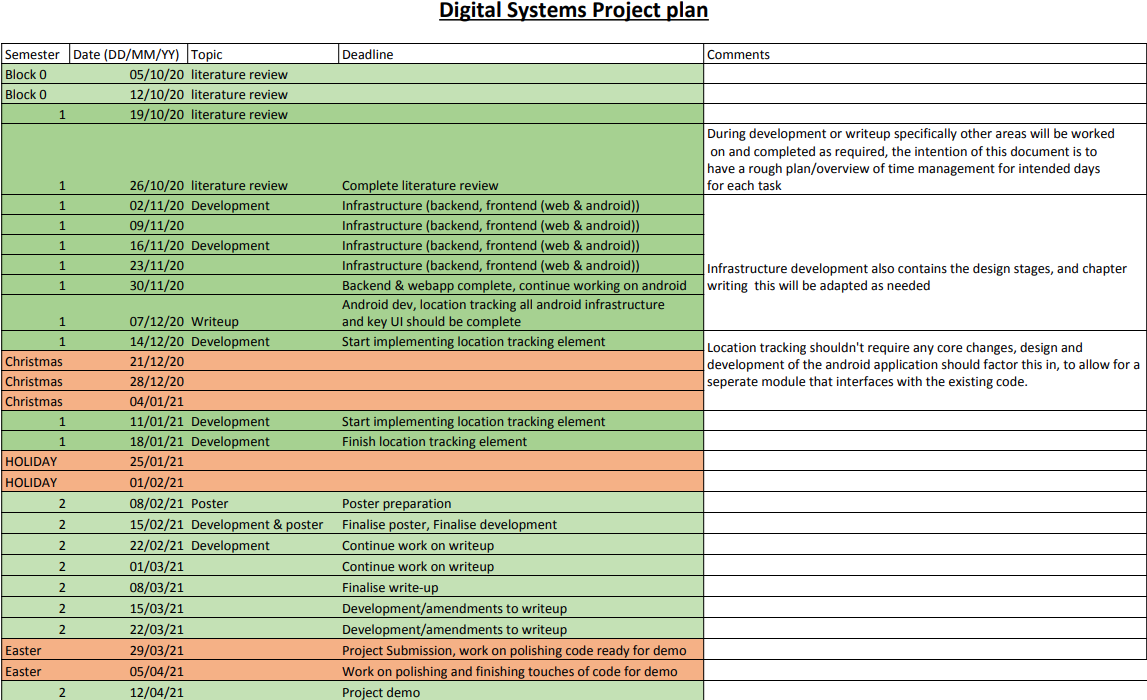
\includegraphics[width=\linewidth]{./images/planning/projectplan.png}\\
	\caption{Initial Project Plan}
	\label{fig:projlan}
\end{figure}

\subsubsection{Development Tools}
Version control is important as part of any project, as such a repository will be made in order to manage the project and ensure error's that are introduced can be reverted as well as having a rough log of the work and progress that has happened throughout development. Git is the current industry standard for version control so this system will be used, a remote repository will be stored on a personal github page.\\

There are many IDE's that exist for a range of purposes. The author is most familiar with the Jetbrains Toolsets such as GoLand and Webstorm, Android studio is also based of the community edition of this. As such the Jetbrains projects will be the IDE of choice for development. However it's important to use a build system for each project in order to not tie the project to a specific IDE so the build model can be changed in the future.


